\documentclass[fleqn]{exam}

\usepackage{fullpage}
\usepackage{enumerate}
\usepackage{unitsdef} 
\usepackage{graphicx}
\usepackage[fleqn]{mathtools}
\usepackage{cancel}
\usepackage{polynom}
\usepackage{float}
\usepackage{mdwlist}
\usepackage{booktabs}
\usepackage{cancel}
\usepackage{polynom}
\usepackage{caption}

\setlength{\mathindent}{.5 cm}

\everymath{\displaystyle}

% \begin{figure}[H]
%   \centering
%   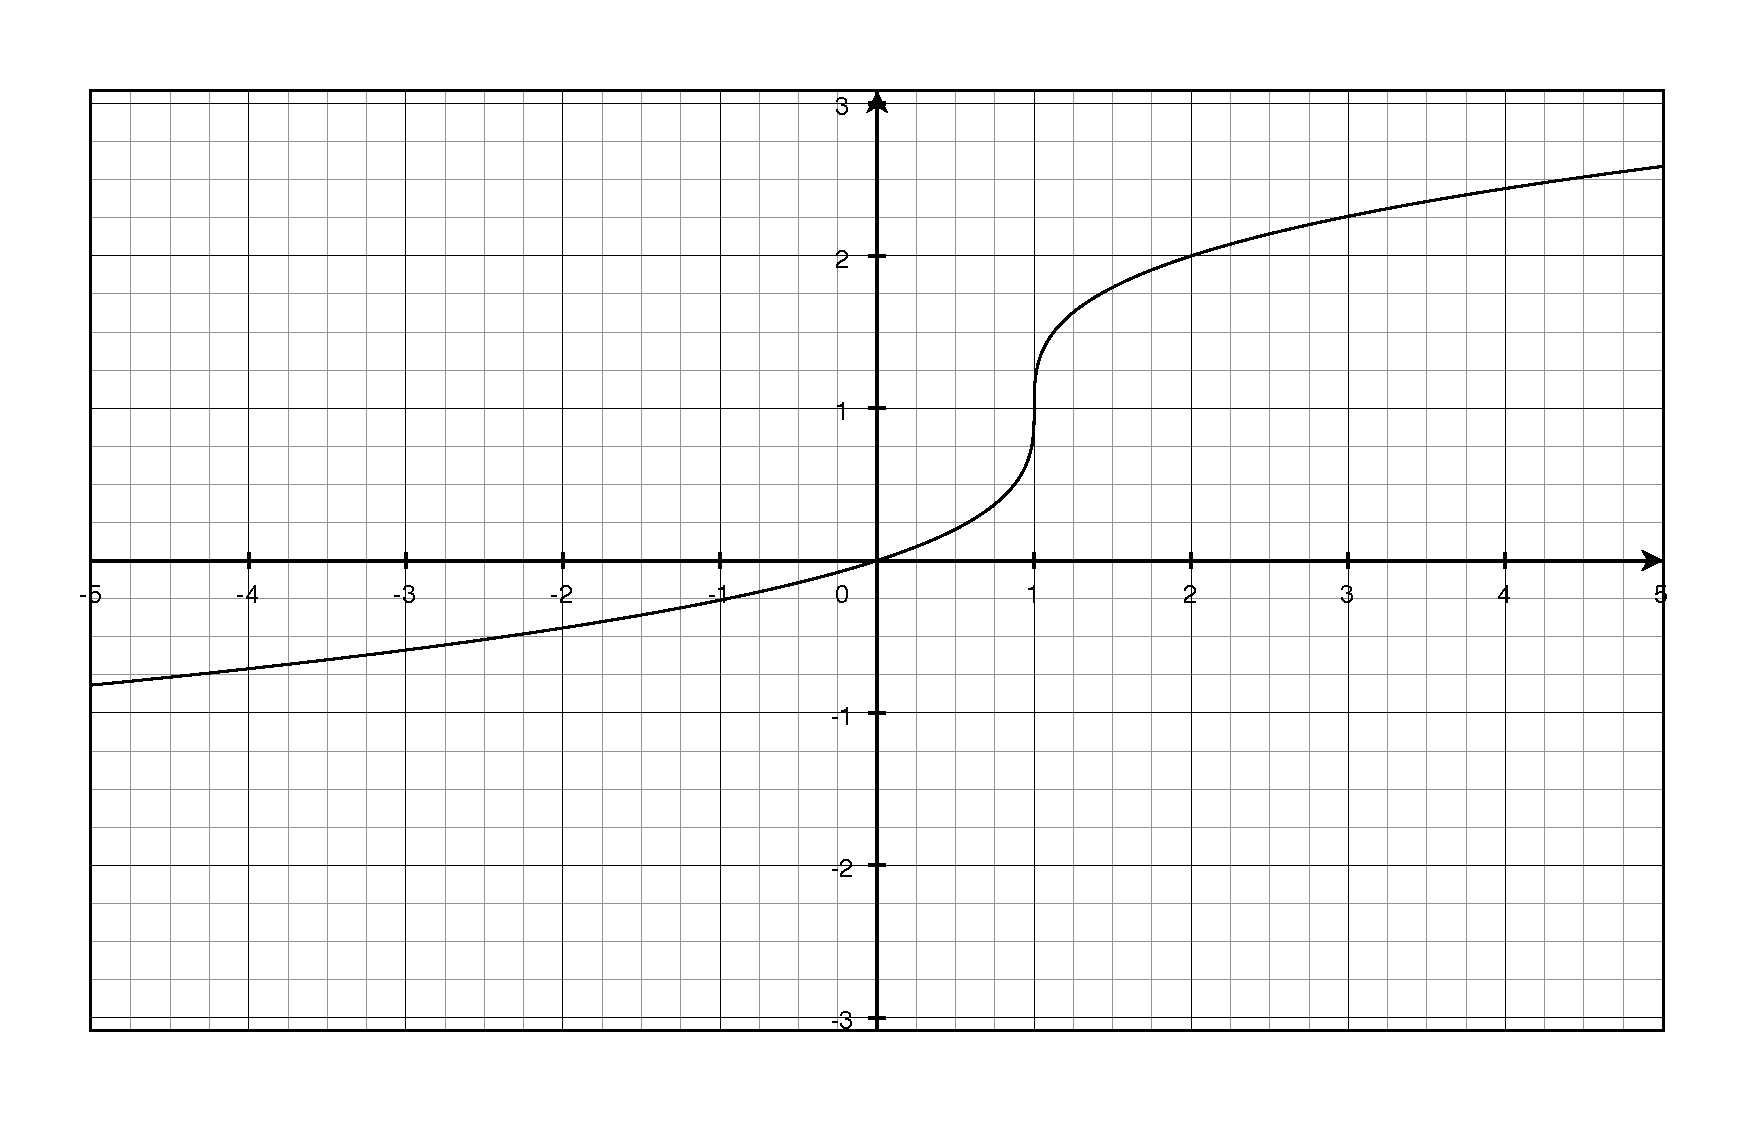
\includegraphics[scale=.3]{question7.eps}
%   \caption*{Question 7}
% \end{figure}

% \begin{tabular}{cc}
% \toprule
% period & amplitude \\
% \midrule
%   $\pi$ & $2$ \\
% \bottomrule
% \end{tabular}

\newunit{\inch}{in}
\newunit{\mile}{mile}
\newunit{\foot}{ft}
\newunit{\knot}{knot}
\newunit{\gallon}{gallon}

\printanswers

\ifprintanswers 
\usepackage{2in1, lscape} 
\fi

\title{Math 263a \\ Homework 11}
\date{April 4, 2012}

\begin{document}

\maketitle

\ifprintanswers
\else
\section{Administrative}
\begin{itemize*}
  \item April 11---review Chapters 2-3
  \item April 18---exam Chapters 2-3
\end{itemize*}

\fi

\section{Homework}

\begin{itemize*}
  \item Read Section 3.10
  \item pp. 166-167: 5-9, 11, 13, 15-18, 21, 24-25, 27-28, 33
\end{itemize*}

\section{Extra Credit}
Page 167, problem 35

\begin{align*}
  m &= m_0 \left( 1 - \cfrac{v^2}{c^2} \right)^{-1/2} \\
  dm &= \cfrac{-m_0}{2} \cdot \left( 1 - \cfrac{v^2}{c^2} \right)^{-3/2} \cdot \cfrac{-2v}{c^2} \cdot dv \\
     &= \cfrac{m_0v \cdot dv}{c^2 \left( 1 - \cfrac{v^2}{c^2} \right)^{3/2}} \\
\end{align*}
\begin{align*}
  \frac{dm}{m} &= \frac{m_0v \cdot dv}{c^2 \left( 1 - \cfrac{v^2}{c^2} \right)^{3/2}} 
                   \cdot \frac{\left( 1 - \cfrac{v^2}{c^2} \right)^{1/2}}{m_0} \\
                &= \frac{v \cdot dv}{c^2 \left( 1 - \cfrac{v^2}{c^2} \right)} \\
                &= \frac{v \cdot dv}{c^2 -v^2} \\
                &= \frac{(0.9c)(.02c)}{c^2 - (0.9c)^2} \\
                &= \frac{0.018c^2}{0.19c^2} \\
                &\approx 0.095 \\
                &= 9.5 \% \\
\end{align*}

\ifprintanswers

\section{Section 3.10}

\begin{description}
\item[5]
\begin{align*}
  y &= (\sin x + \cos x)^3 \\
  dy &= 3 (\sin x + \cos x)^2 (\cos x - \sin x) dx \\
\end{align*}

\item[6]
\begin{align*}
  y &= (\tan x + 1)^3 \\
  dy &= 3 (\tan x + 1)^2 \sec^2 x \cdot dx \\
\end{align*}

\item[7]
\begin{align*}
  y &= (7x^2 + 3x - 1)^{-3/2} \\
  dy &= - \frac{3}{2} (7x^2 + 3x - 1)^{-5/2} (14x + 3) dx \\
\end{align*}

\item[8]
\begin{align*}
  y  &= (x^{10} + \sqrt{\sin 2x})^2 \\
  dy &= 2(x^{10} + \sqrt{\sin 2x}) \left(10x^9 + \frac{1}{2} (\sin 2x)^{-1/2} \cdot 2 \cdot \cos 2x \right) dx \\
     &= 2(x^{10} + \sqrt{\sin 2x}) \left(10x^9 + \frac{\cos 2x}{\sqrt{\sin 2x}} \right) dx \\
\end{align*}

\item[9]
\begin{align*}
  F(t) &= (t - 2)^{2/5} \\
  dF   &= \frac{2}{5} (t - 2)^{-3/5} dt \\
\end{align*}

\item[11]
\begin{align*}
  y &= x^3 \\
  dy &= 3x^2 dx \\
\end{align*}

\begin{enumerate}[a]
\item
$x = 0.5$; $dx = 1$
\begin{align*}
  dy &= 3 \cdot \left(\frac{1}{2} \right)^2 \cdot 1 \\
     &= 0.75 \\
\end{align*}

\begin{figure}[H]
  \centering
  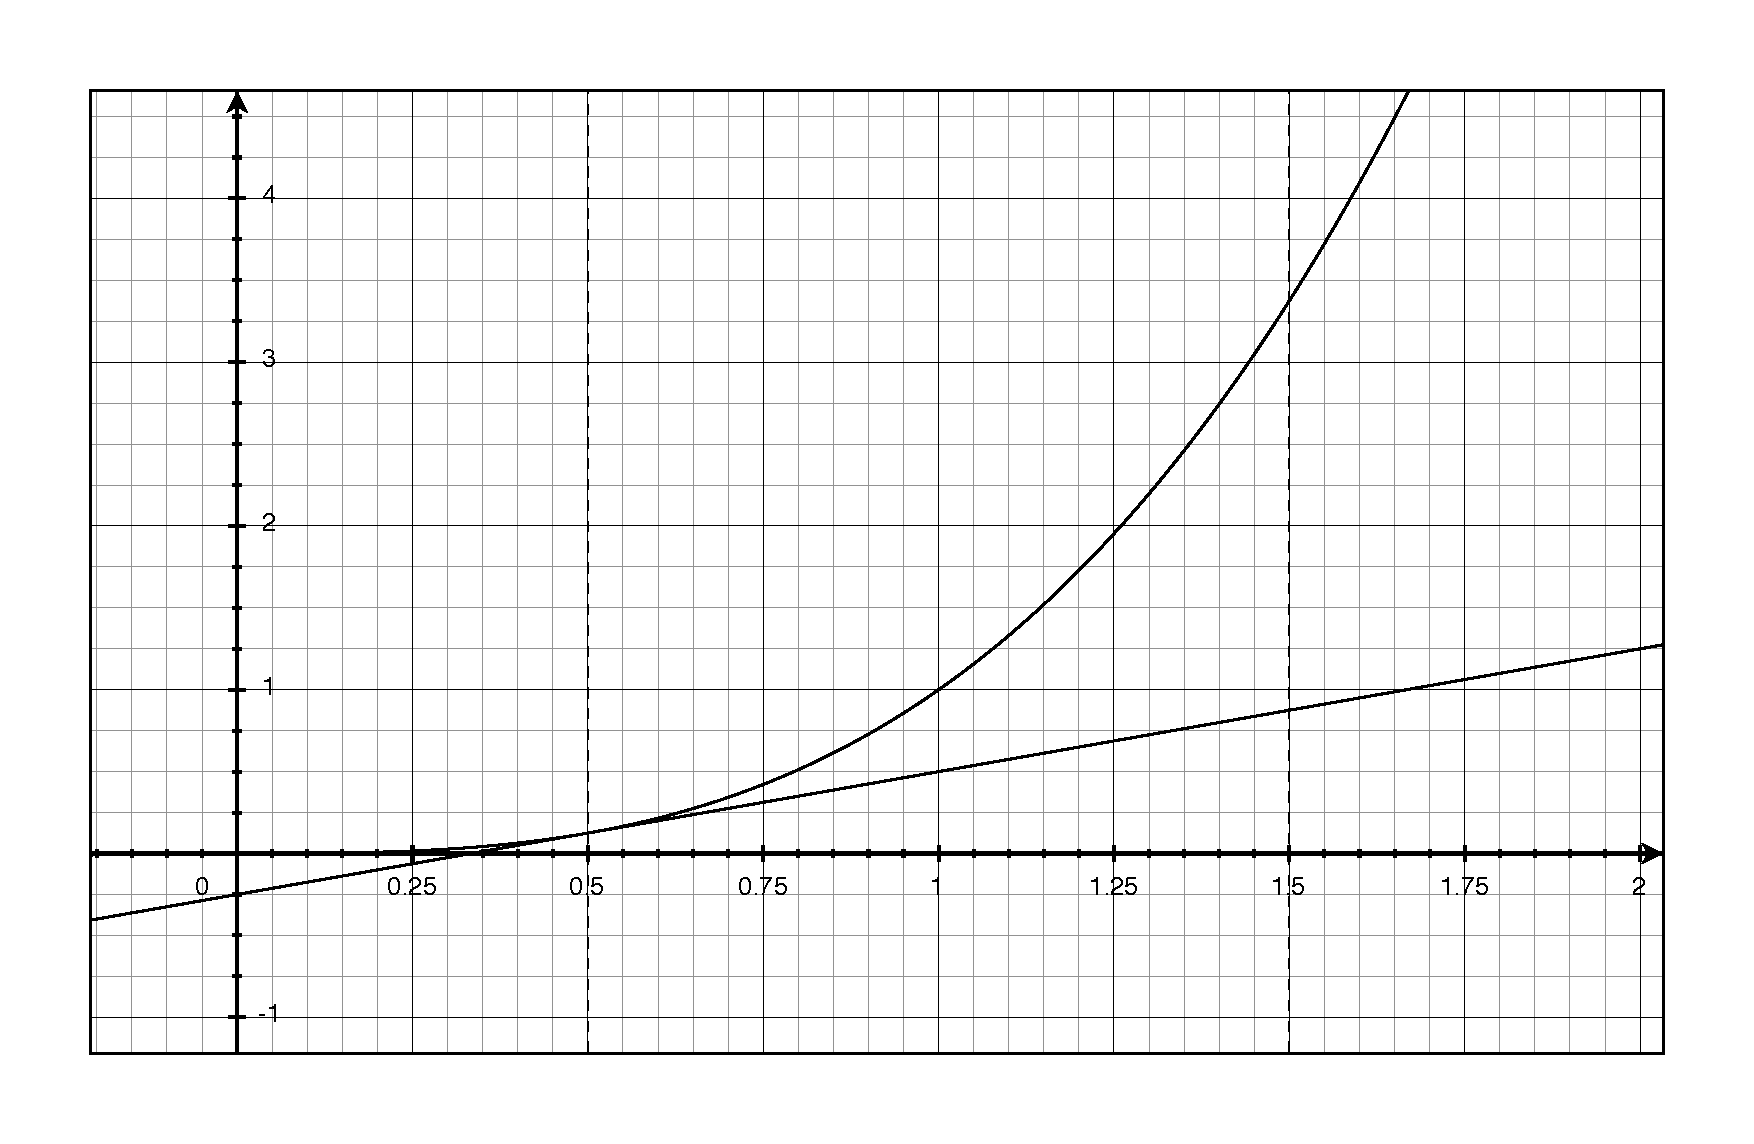
\includegraphics[scale=.3]{problem_11a.eps}
  \caption*{Problem 11a}
\end{figure}

\item
$x = 1$; $dx = \frac{3}{4}$
\begin{align*}
  dy &= 3 \cdot 1 \left(\frac{3}{4} \right) \\
     &= 2.25 \\
\end{align*}


\begin{figure}[H]
  \centering
  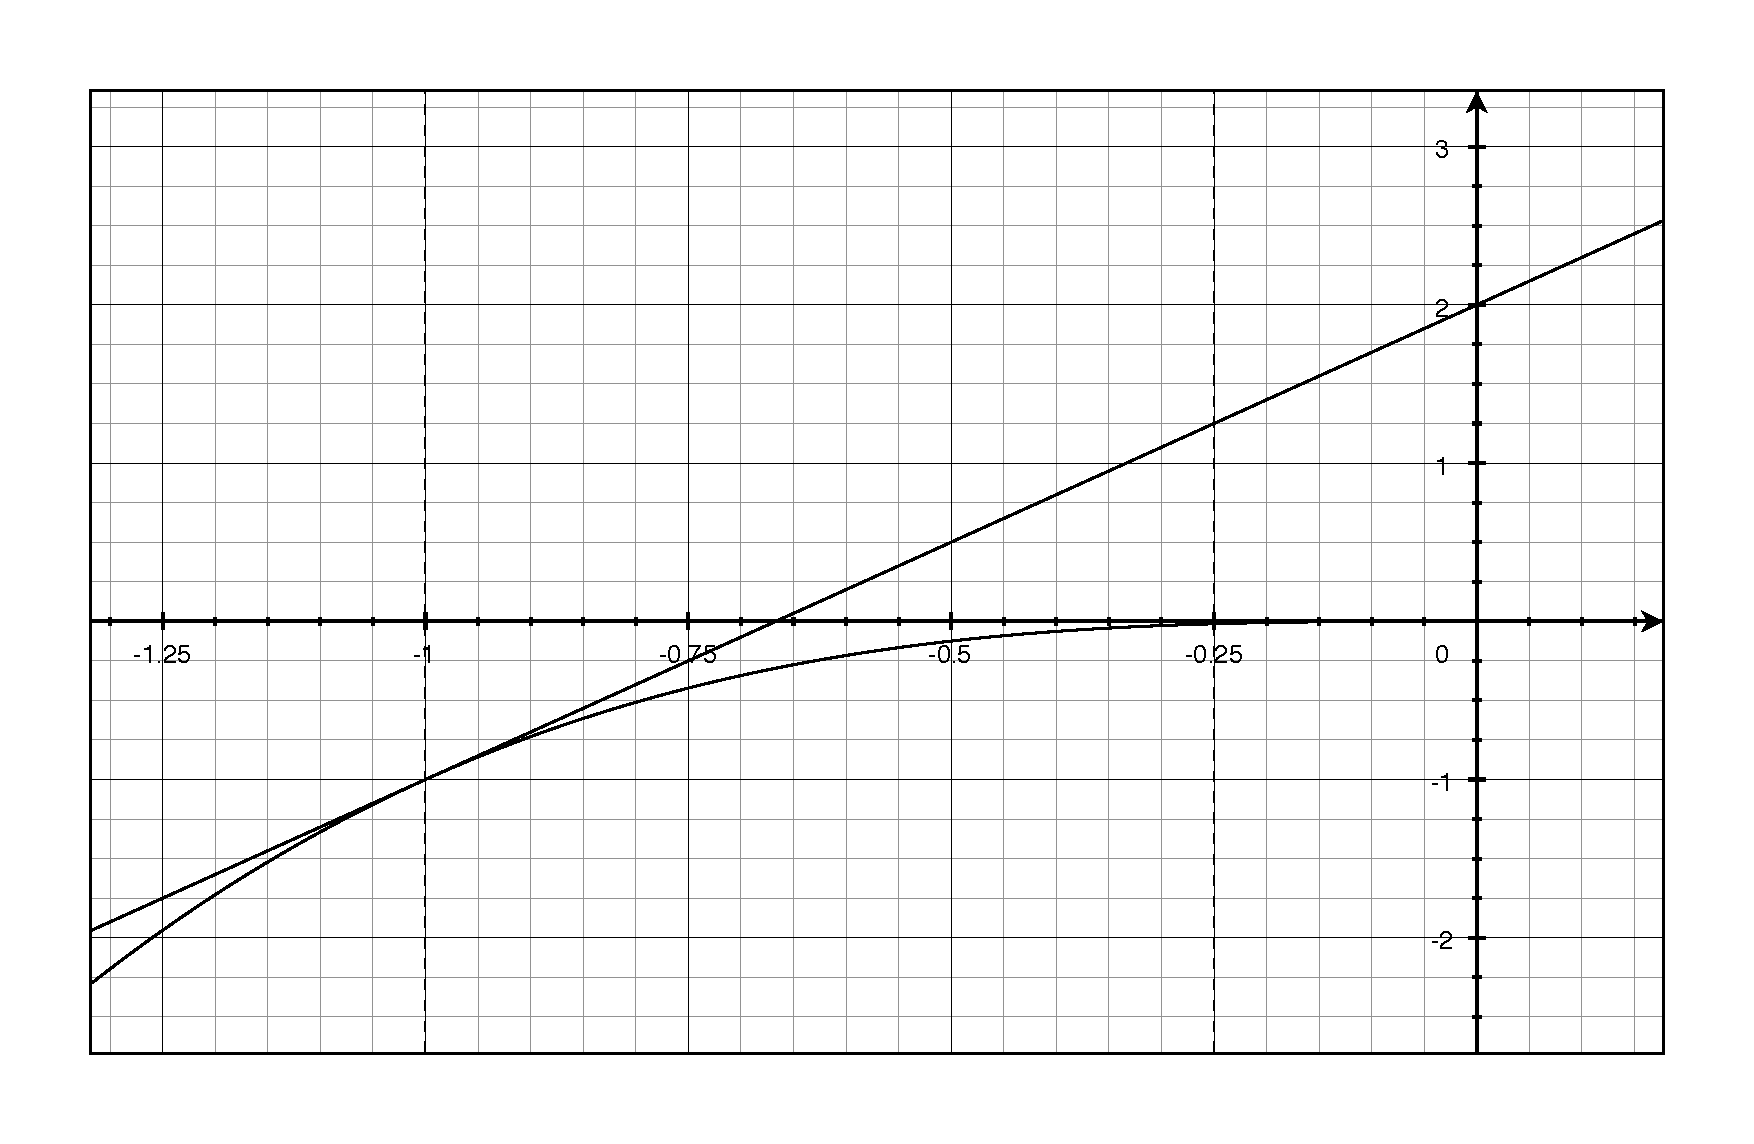
\includegraphics[scale=.3]{problem_11b.eps}
  \caption*{Problem 11b}
\end{figure}

\end{enumerate}

\item[13]
\begin{enumerate}[a]
\item
\[
  \Delta y = (1.5)^3 - (0.5)^3 = 3.25
\]

\item
\[
  \Delta y = (-0.25)^3 - (-1)^3 \approx 0.9844
\]

\end{enumerate}

\item[15]
\begin{align*}
  y &= x^2 - 3 \\
  dy &= 2x \cdot dx \\
\end{align*}

\begin{enumerate}[a]
\item
\begin{align*}
  dx &= 2 \cdot 2 \cdot 0.5 = 2 \\
  \Delta x &= 2.5^2 - 3 - (2^2 - 3) = 2.25 \\
\end{align*}

\item
\begin{align*}
  dx &= 3 \cdot 2 \cdot (-0.12) = -0.72 \\
  \Delta x &= 2.88^2 - 3 - (3^2 - 3) \approx -0.706 \\
\end{align*}

\end{enumerate}

\item[16]
\begin{align*}
  y &= x^4 + 2x \\
  dy &= (4x^3 + 2) \cdot dx \\
\end{align*}

\begin{enumerate}[a]
\item
\begin{align*}
  dy &= (4 \cdot 2^3 + 2) \cdot 1 = 34 \\
  \Delta y &= (3^4 + 2 \cdot 3) - (2^4 + 2 \cdot 2) = 67 \\
\end{align*}

\item
\begin{align*}
  dy &= (4 \cdot (2)^3 + 2) \cdot 0.005 \approx 0.17\\
  \Delta y &= (2.005^4 + 2 \cdot 2.005) - (2^4 + 2 \cdot 2) \approx 0.1706 \\
\end{align*}

\end{enumerate}

\item[17]
\begin{align*}
  y &= x^{1/2} \\
  dy &= \frac{dx}{2 \sqrt{x}} \\
  \\
  dy &= \frac{2}{2 \sqrt{400}} \\
     &= \frac{1}{20} \\
  \\
  \sqrt{402} &\approx 20 + \frac{1}{20} = 20.05
\end{align*}

\item[18]
\begin{align*}
  y &= x^{1/3} \\
  dy &= \frac{dx}{3 \sqrt[3]{x^2}} \\
  \\
  dy &= \frac{-0.09}{3 (\sqrt[3]{27})^2} \\
     &= \frac{-0.09}{27} \\
     &\approx -0.00333 \\
  \\
  \sqrt[3]{26.91} &\approx 3 - 0.00333 \approx 2.997
\end{align*}

\item[21]
\begin{align*}
  V  &= \frac{4}{3} \pi r^3 \\
  dV &= 4 \pi r^2 dr \\
  \\
  dV &= 4 \pi \cdot 5^2 \cdot 0.125 \cm^3 \\
     &\approx 39.27 \cm^3 \\
\end{align*}

\item[24]
\begin{align*}
  V  &= \pi r^2h \\
  dV &= 2 \pi rh dr \\
  \\
  dV &= 2 \pi \cdot 72 \cdot 96 \cdot 0.05 \inch^3 \\
     &\approx 2,171 \inch^3 \\
     &\approx 9.4 \gallon \\
\end{align*}

\item[25]
\begin{align*}
  C  &= 2 \pi r \\
  dC &= 2 \pi \cdot dr \\
  \\
  dC &= 2 \pi \cdot 2 \foot \\
     &\approx 12.57 \foot \\
\end{align*}

\item[27]
\begin{align*}
  V  &= \frac{4}{3} \pi r^3 \\
  dV &= 4 \pi r^2 dr \\
  \\
  dV &= 4 \pi \cdot 10^2 \cdot 0.05 \cm^3 \\
     &\approx 63 \cm^3 \\
  \\
  V &= 4,189 \pm 63 \cm^3
\end{align*}

\item[28]
\begin{align*}
  V  &= \pi r^2 h \\
  dV &= 2 \pi rh \cdot dr \\
  \\
  dV &= 2 \pi \cdot 3 \cdot 12 \cdot 0.0025 \inch^3 \\
     &\approx 0.565 \inch^3 \\
  \\
  V &= 339 \pm 0.565 \inch^3
\end{align*}

\item[33]
\begin{align*}
  V  &= \frac{4}{3} \pi r^3 + \pi r^2 h \\
  dV &= (4 \pi r^2 + 2 \pi r) \cdot dr \\
  \\
  dV &= (4 \pi \cdot 10^2 + 2 \pi \cdot 10 \cdot 100) \cdot 0.1 \cm^3 \\
     &\approx 754 \cm^3 \\
\end{align*}

\end{description}


\else

\vspace{8 cm}

{\em From this point forth we shall be leaving the firm foundation of fact and journeying together
through the murky marshes of memory into thickets of wildest guesswork.}

\vspace{.2 cm}

\hspace{1 cm} --Albus Dumbledore

%% {\em When we are unhurried and wise, we preceive that only great and worthy things have any permanant and absolute
%% existence,---that petty fears and petty pleasures are but the shadow of reality.}

%% \vspace{.2 cm}

%% \hspace{1 cm} --Henry David Thoreau

\fi

\end{document}

